%\documentclass[a4paper,12pt,oneside,draft]{article}
\documentclass[a4paper,12pt,oneside]{article}

% In the original writelatex tamplate
\usepackage[english]{babel}
\usepackage[utf8]{inputenc}
\usepackage{amsmath}
\usepackage{graphics}
\usepackage[colorinlistoftodos]{todonotes}

% By LoCigno
\usepackage{times}
\usepackage{graphicx}
\usepackage{subfigure}
\usepackage{csvsimple}
\usepackage{color}
\usepackage{url}
\usepackage{hyperref} 
\usepackage{cleveref}

% By Davide
\usepackage{comment}
\usepackage{booktabs}
\usepackage{color}

%Variables macros
\newcommand{\DefineVar}[2]{%
  \expandafter\newcommand\csname var-#1\endcsname{#2}%
} 
\newcommand{\var}[1]{\csname var-#1\endcsname}

\usepackage{courier}
\newcommand{\mono}[1]{\texttt{#1}}

\title{Controller design for Lego Mindstorm motor}

\author{Diego Verona, Aliaksandr Siarohin, Mattia Digilio}

\date{\today}

% By Diego
\newtheorem{thm}[equation]{Theorem}
\usepackage[outdir=./]{epstopdf}
\usepackage{float}

\begin{document}
%\maketitle
\makeatletter  % populates \@title, \@author, \@date
\begin{titlepage}
      \centering
      ~~~~~~~~~~~~~\\[-30mm]
      
\includegraphics[keepaspectratio=true, width=7cm]{bg_eng_1r.jpg} \\[10mm]

     {
     \large \bfseries Master Degree in Computer Science\\[3mm] 
     Applied Robotics\\[3mm]
     AA 2015-2016
     }\\[10mm]

     %--------------------------------
     % Set the title, author, and date
     % 

     \vspace{0.5cm}
     {
     \Large \bfseries \textcolor{blue}{\@title} \par
     }
     \vspace{0.5cm}
%      {
%      \large {Group N. 1} \par
%      }
     \vspace{0.2cm}

     {\large {\@author}}
     \\ \vspace{.2cm}
     \@date

     \vspace{0.6cm}

    %-----------------------------------

\begin{abstract}

\textit{
  Report for the third assignment on Applied robotics: design and implement a simple model of vehicle that can go straight without additional sensors for the Lego NXT.\\In this report we show model of a vehicle, describing its properties and its digital implementation.
}


\end{abstract}

\end{titlepage}

\section{General definition}


\section{Design of vehicle}
\subsection{Vehicle requirments}
The vehicle should go statight without additional sensors and human interation, and it should change its velocity according to the covered distance. The model of the robot should have at least three wheels and two motors, one wheel is free, and the two other should be controlled by the motors. 
\subsection{Lego structure}
The design of our lego robot can be found in the following pictures: \cref{fig:back}, \cref{fig:front}, 
\cref{fig:left}.
\subsection{Controller design}
We have 2 motors, so for every of them we create a separate controller and we called them "inner". We have also a controller called "outer" that ajust the direction of the vehicle, balancing  motor powers. The overall structure can be found in: \cref{fig:diagram}

Velocity of the vehicle:
\begin{equation}
\text{velocity} = R \frac{velocity_A + velocity_B}{2} 
\end{equation}

Where R - is radius of the wheel. And $velocity_A$, $velocity_B$ is angular velocity of the motors. 

And the direction of the vehicle is:
\begin{equation}
\text{direction} = R \frac{velocity_B - velocity_A}{L}
\end{equation}

Where L is the distance between wheels. The direction should be 0 in order for vehicle to move straight.


\subsection{Controller implementation}
The main task is runned every 5ms and do this operations:
\begin{enumerate}
\item Compute current velocities of the motors using exponential avearage.
\item Compute vehicle velocity and its direction
\item Compute difference in motor velocities
\item Use this difference to compute new velocity for the motors
\item Compute new motors power based on the new velocity using controller from assigment 2
\end{enumerate}
\section{Conclusion}

In this assignment we designed a simple vehicle structure and implemented it usign Lego NXT.


\begin{figure}
	\centering
	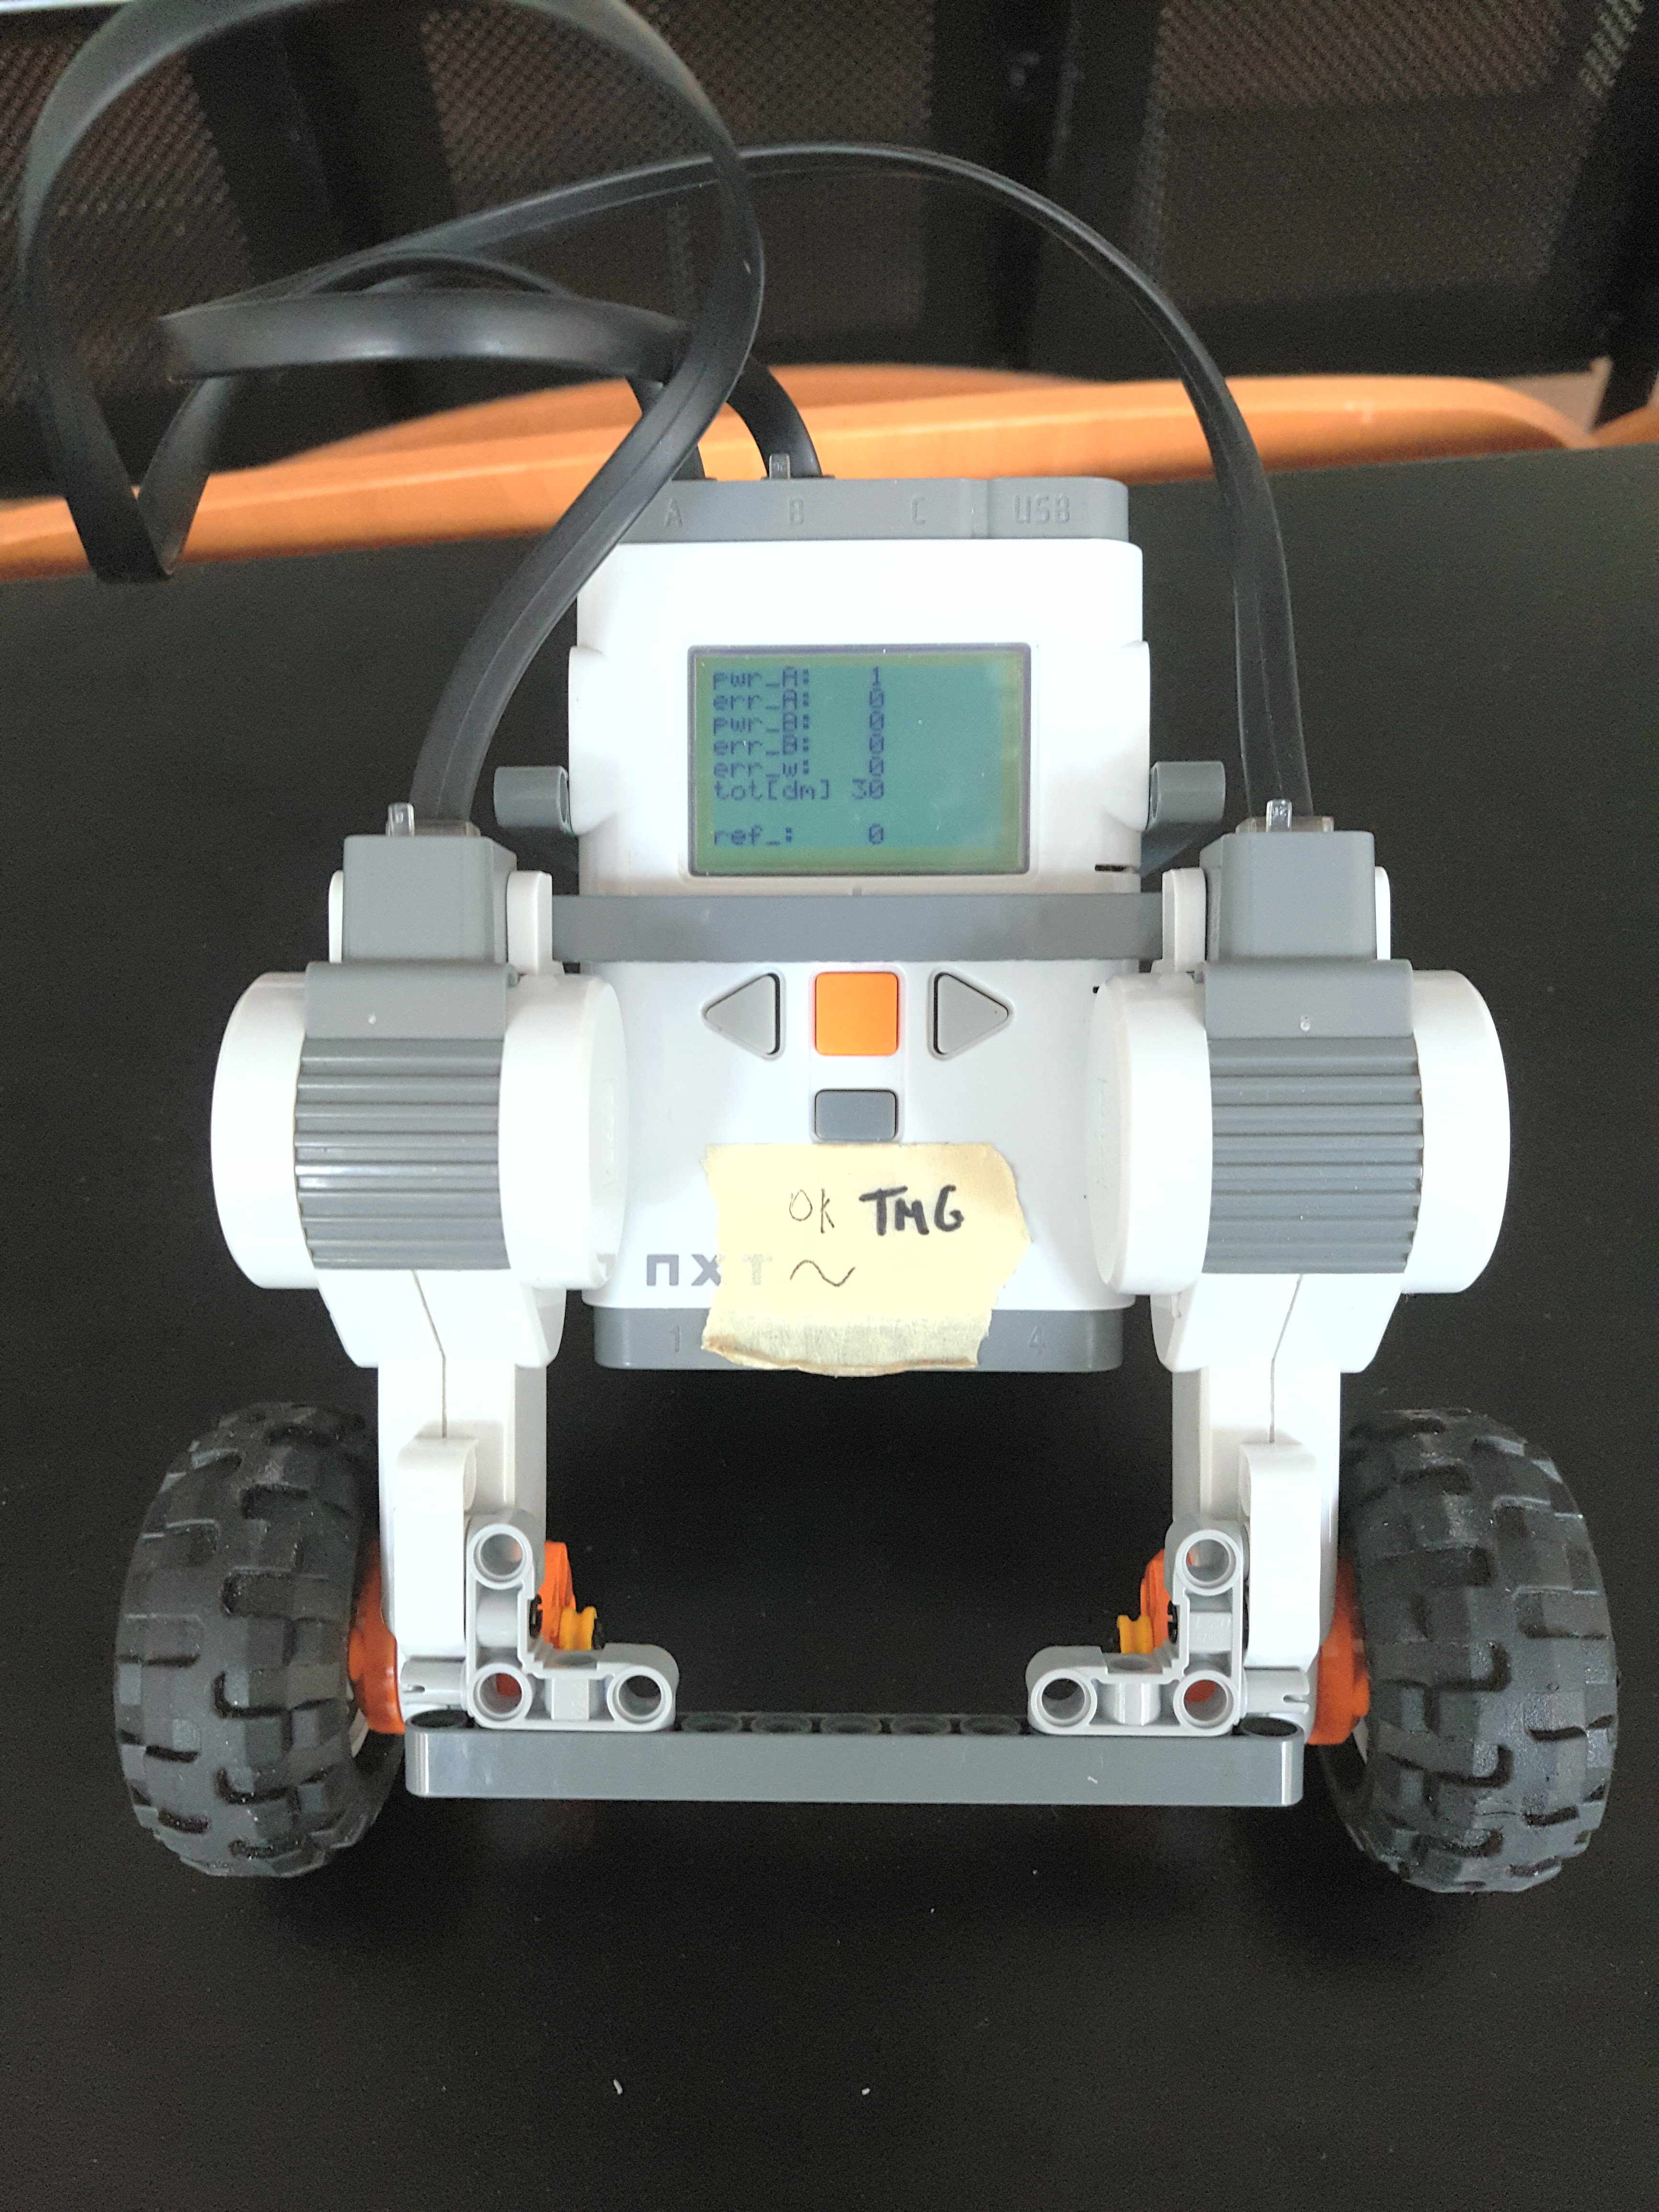
\includegraphics[width=\columnwidth]{nxtImages/1.jpg}
	\caption{Back side}
	\label{fig:back}
\end{figure}
\begin{figure}
	\centering
	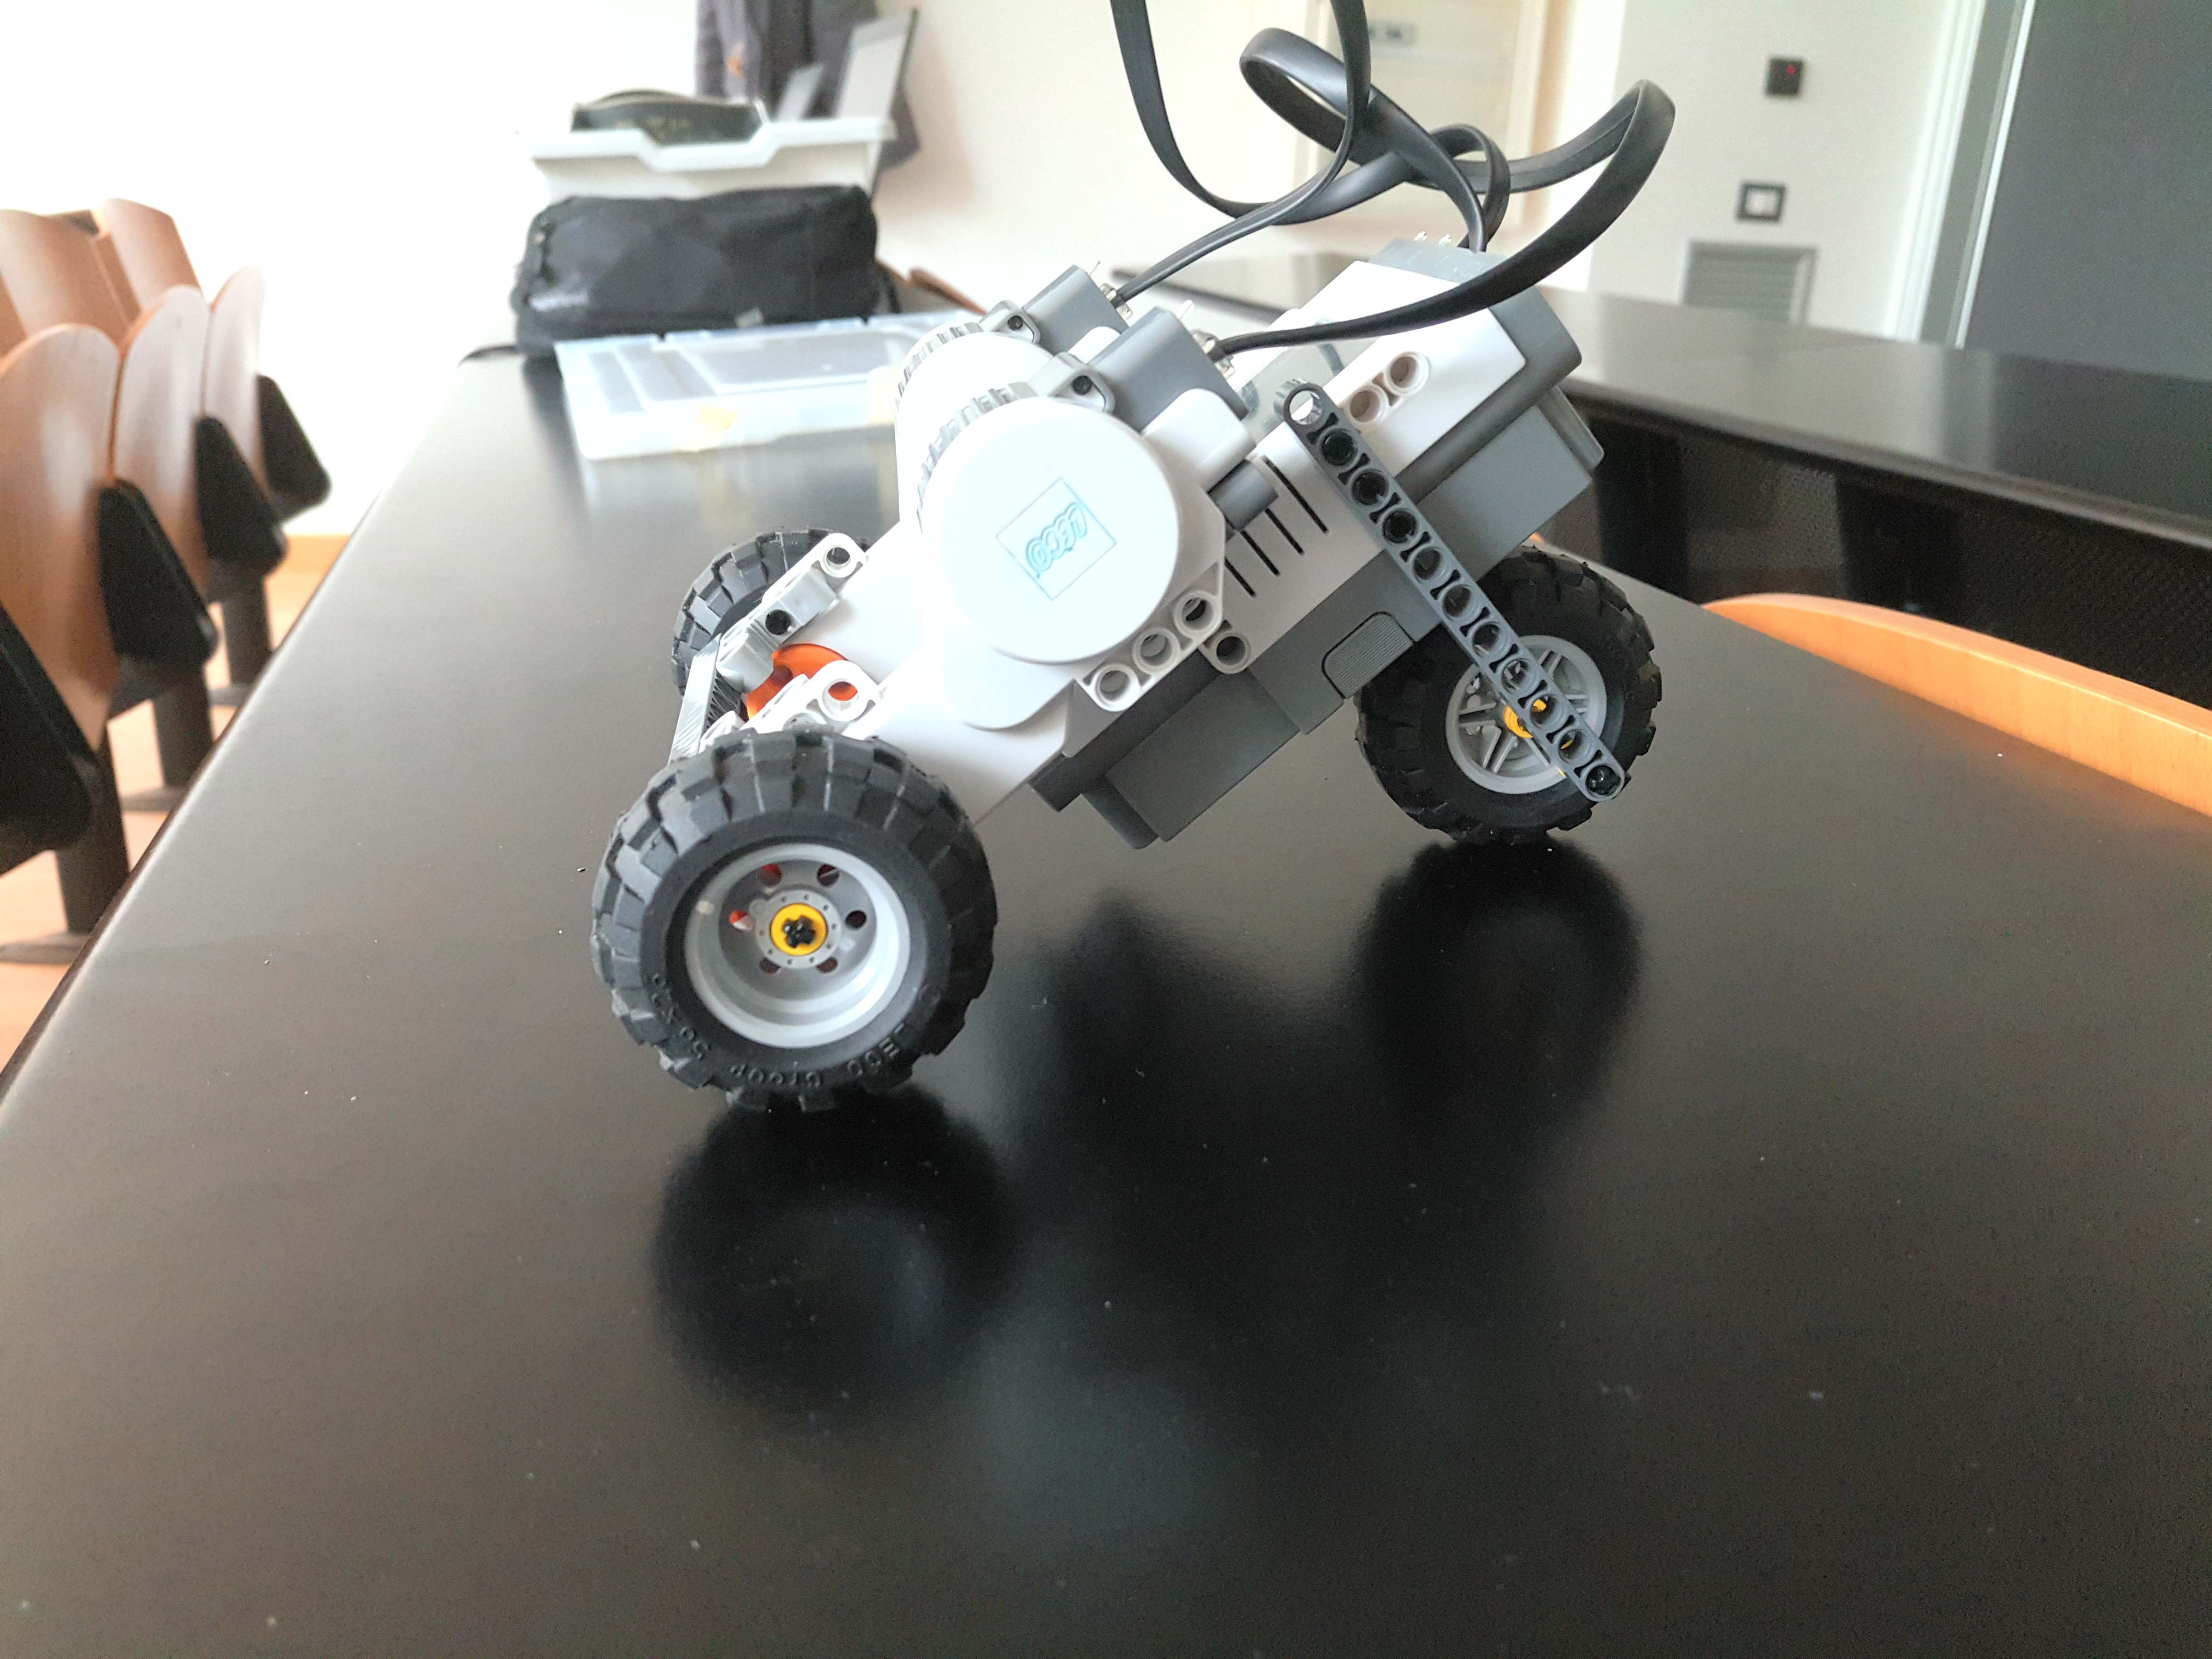
\includegraphics[width=\columnwidth]{nxtImages/2.jpg}
	\caption{Left side}
	\label{fig:left}
\end{figure}
\begin{figure}
	\centering
	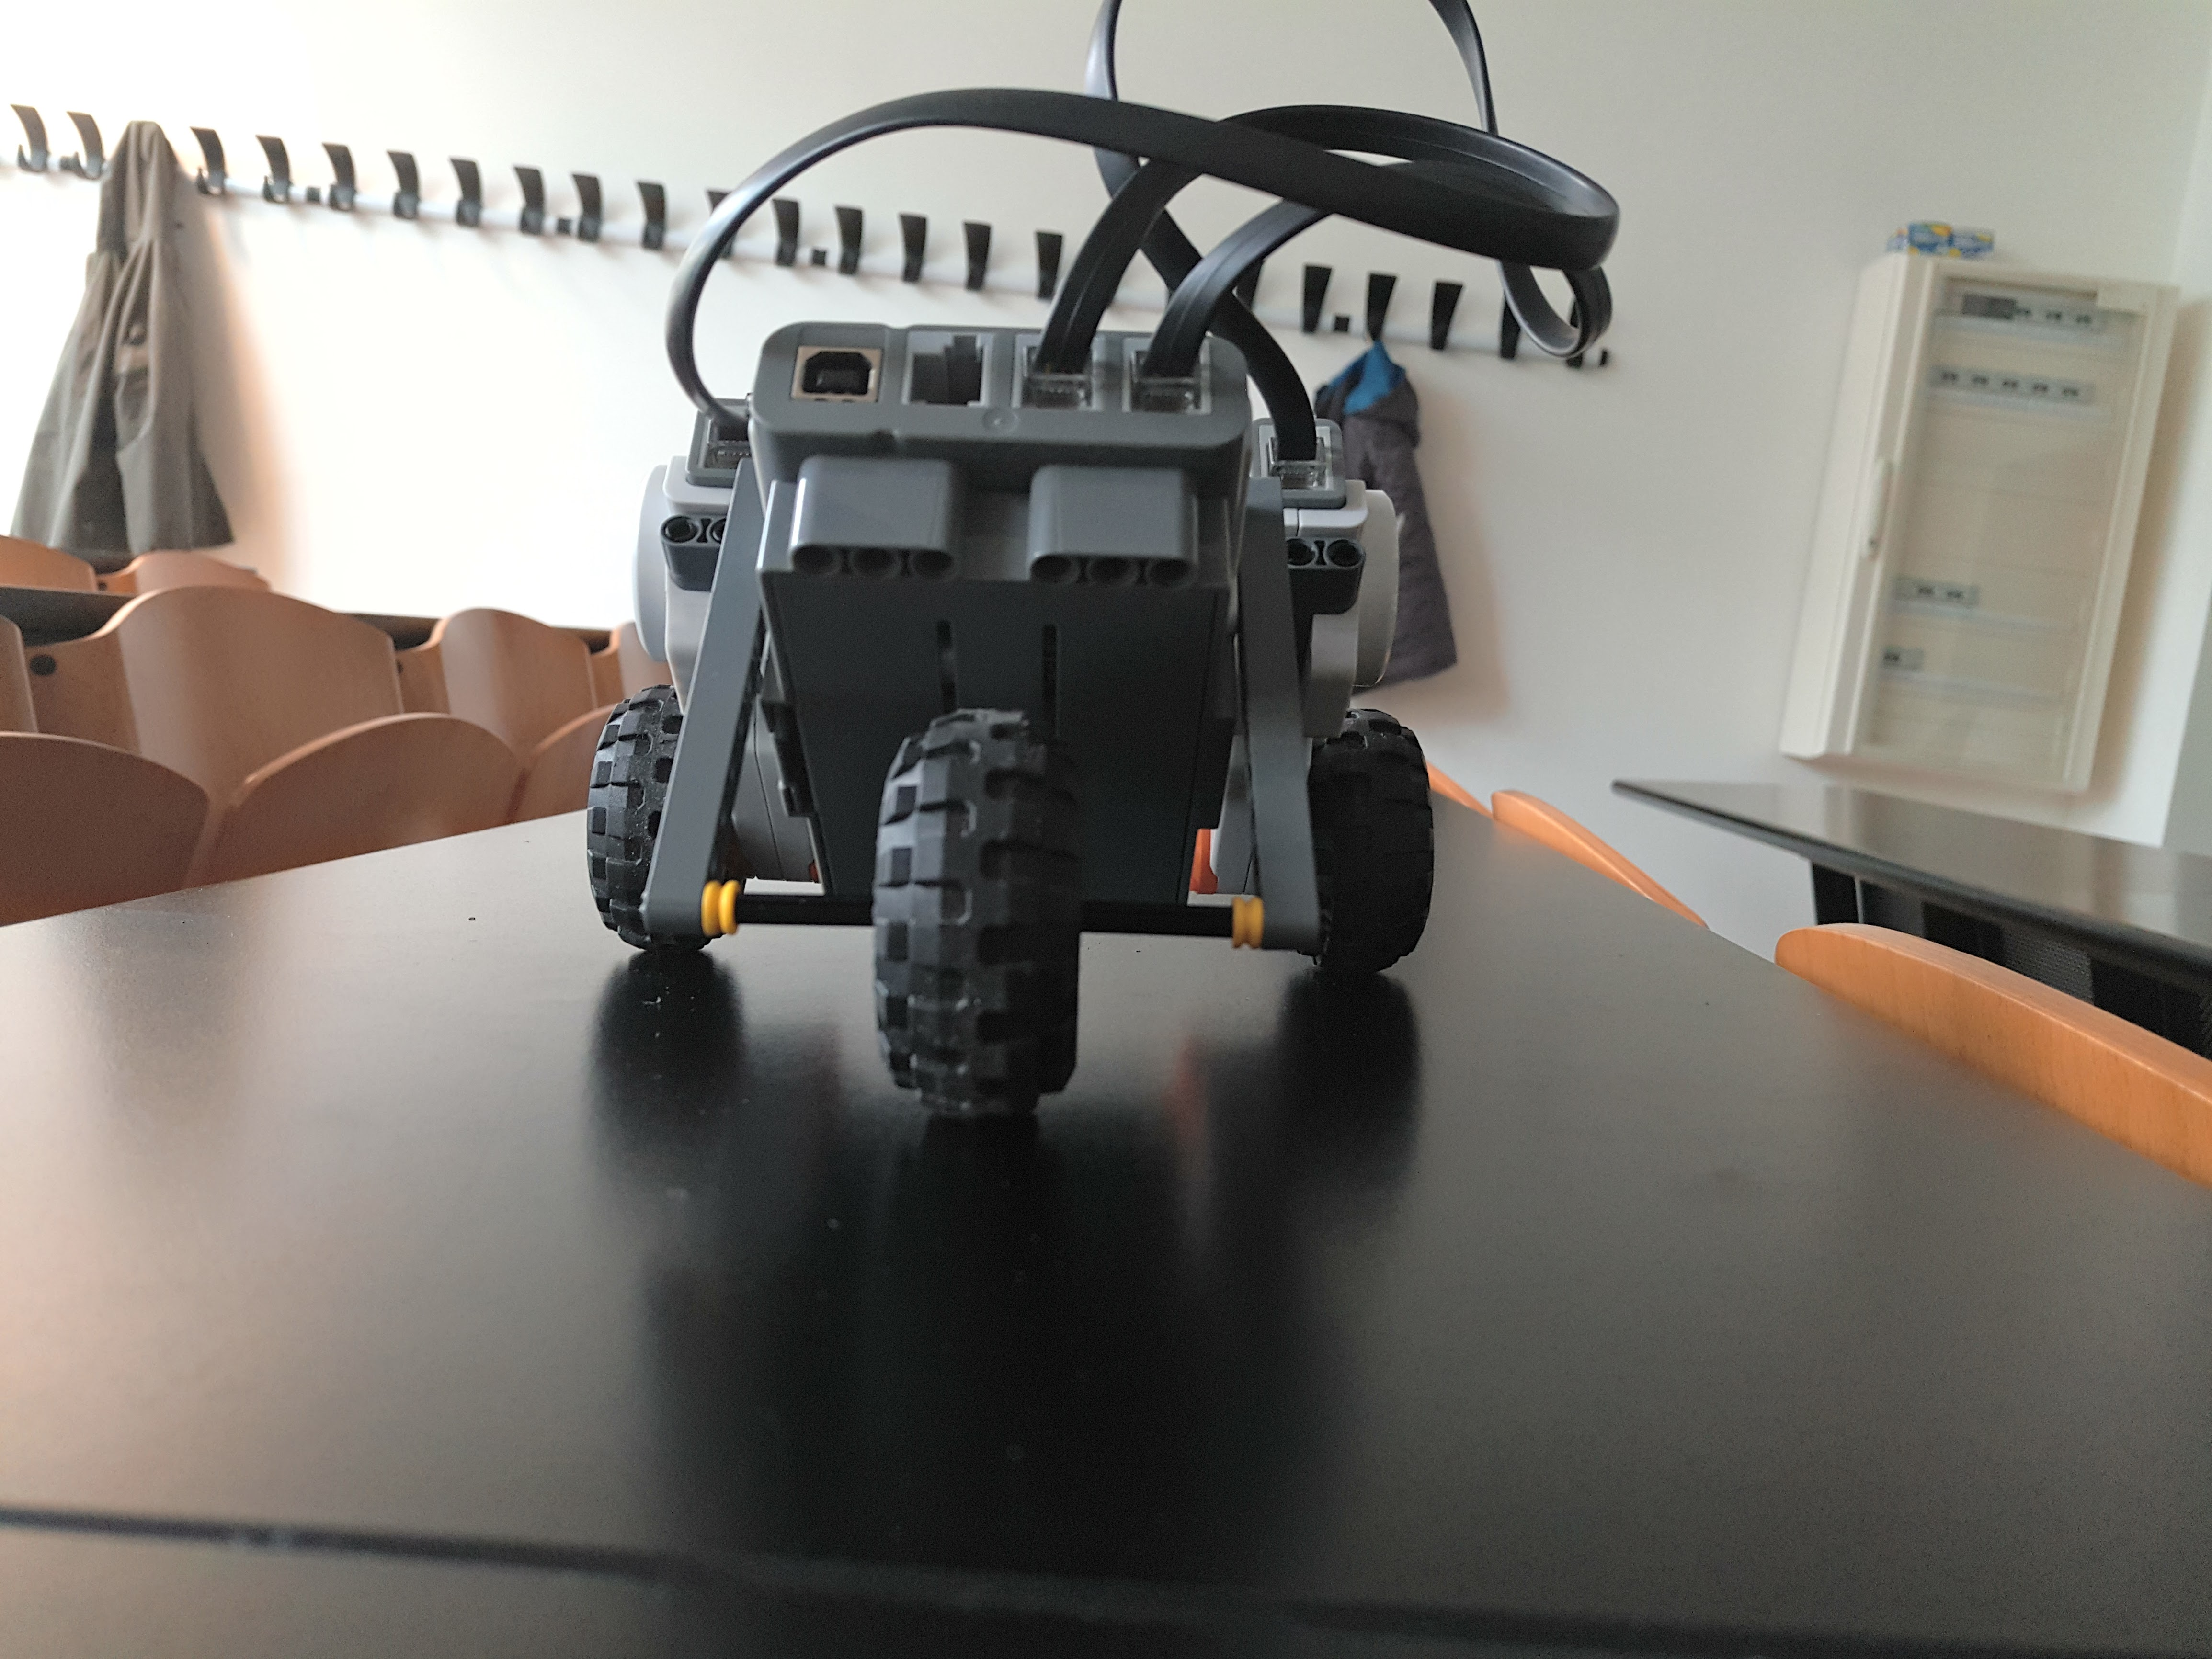
\includegraphics[width=\columnwidth]{nxtImages/3.jpg}
	\caption{Front side}
	\label{fig:front}
\end{figure}
\begin{figure}
	\centering
	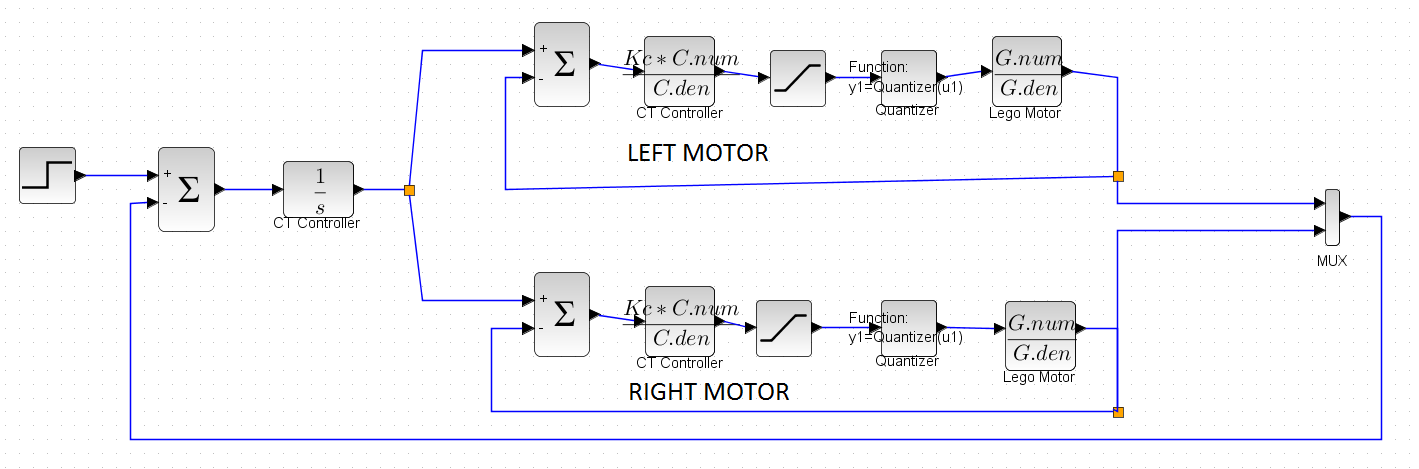
\includegraphics[width=\columnwidth]{vehicle.png}
	\caption{Structure of vehicle controller}
	\label{fig:diagram}
\end{figure}


\end{document}